\section{MTBF und Reliability}\label{sec:MTBF}
Es gibt viele Ursachen, welche zu einem Ausfall elektronischer Komponenten in einem System, führen können. Laut dem technischen Bericht \cite{AIP} ist in 50\% der Fälle die Temperatur der Komponenten für einen Ausfall verantwortlich. Dies liegt an den unterschiedlichen thermischen Ausdehnungskoeffizienten des Materials auf der Platine haben. Durch die unterschiedliche Ausdehnung der Bauteile und der Platine selbst, kommt es zu hohen Belastungen der Lötstellen. Während sich dieser Zyklus wiederholt,  können Risse in den Verbindungen entstehen und ausbreiten. Diese können anschließend zu einem Bruch im elektrischen Stromkreis führen. \cite{AREPA_LifeExpectancy}\\
\begin{wrapfigure}{r}{0.65\textwidth}
    \vspace{-1.2cm}
    \begin{center}
      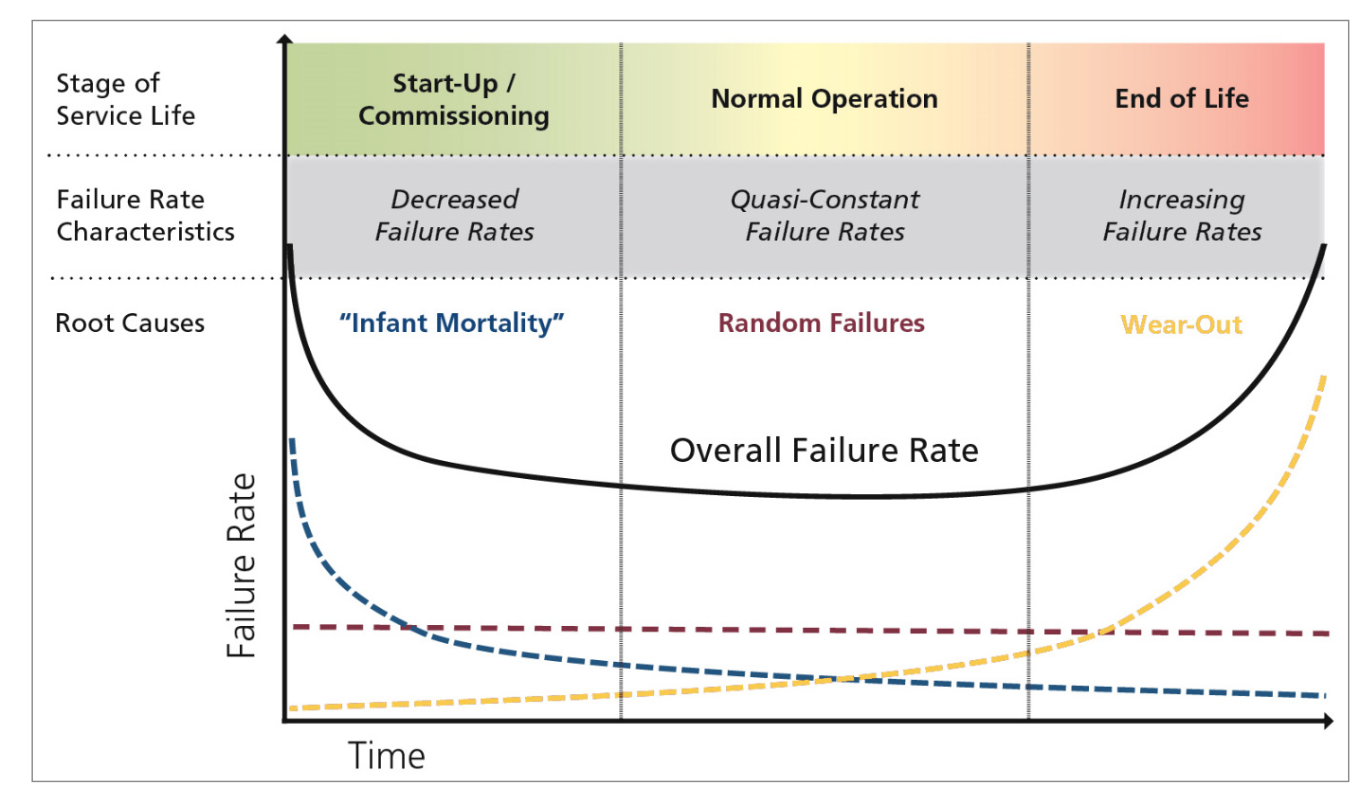
\includegraphics[width=0.64\textwidth]{BathTubCurve}
    \end{center}
    \vspace{-0.5cm}
    \caption{Bathtub Curve \cite{AREPA_LifeExpectancy}}
    \label{fig:BathTubCurve}
    \vspace{-0.5cm}
  \end{wrapfigure}
  Die in Abbildung \ref{fig:BathTubCurve} abgebildete Bathtub-Kurve ist ein Konzept, welches zur Beschreibung der Lebensdauer von elektronischer Komponenten verwendet wird. Dabei kann die Lebenszeit in drei Abschnitte unterteilt werden. Die Bathtub-Kurve beschreibt eine mittlere Betriebsdauer zwischen Ausfällen. Sie weist drei Betriebsphasen auf. 
  In der ersten Phase, bekannt als \textit{Infant Mortality}, kommt es durch Konstruktions-, Produktions- und Werkstoffmängel häufig gleich zu Beginn des Betriebs zu Fehlern und Ausfällen. Geräte, die von diesen Problemen nicht betroffen sind, laufen meist zuverlässig durch die zweite Phase der Kurve, bekannt als \textit{Random Failures}. Hierbei kommt es nur deutlich seltener und vereinzelt zu Ausfällen. Zum Ende der Lebensdauer kommt es, in der \textit{Wear-Out} Phase, durch Alterung und Verschleiß wieder vermehrt zu Ausfällen. \cite{AREPA_LifeExpectancy}\\ 
  Der \ac{mtbf} ist dabei eine statistische Kennzahl, die den durchschnittlichen Zeitraum in Stunden angibt, der zwischen zwei aufeinanderfolgenden Ausfällen einer bestimmten Komponente, eines Systems oder eines Produkts verstrichen is. Dieser weist zudem eine Temperaturabhängigkeit auf. Beispielsweise bei Kapazitäten kann im Durchschnitt gesagt werden: \textit{Eine Erhöhung der Betriebstemperatur um 10°C, führt zu einer Halbierung der Lebenserwartung}. Ein \ac{mtbf} von 100h sagt also aus, dass ein System im Durchschnitt, 100h laufen wird, bevor es zu einem Fehler kommen wird.\cite{MTBFReliability}\\
  Die Zuverlässigkeit (Reliability) eines Gerätes hingegen ist als die Wahrscheinlichkeit definiert, mit der ein System seine beabsichtigten Funktionen für einen festgelegten Zeitraum erfüllen wird. Hat ein System bei 100h eine Zuverlässigkeit von 0.8, so besteht eine 80\% Wahrscheinlichkeit, dass das System nach 100h noch funktioniert.\cite{MTBFReliability}\\
  Die Zuverlässigkeit eines Systems kann über den \ac{mtbf} mit Formel \ref{equ:Reliability} berechnet werden. Dabei ist zu beachten, dass man die Temperaturabhängigkeiten des Systems beachtet.
\begin{align}
    && R(t) &= e^{-\frac{t}{\text{mtbf}}} &&
    \label{equ:Reliability} 
\end{align}
